\newpage

\anonchapter{Лабораторная работа №2}
\setcounter{chapter}{2}

\begin{center}
Определение ширины запрещённой зоны полупроводника \\
(4 часа)
\end{center}

\section{Цель работы}
Определение ширины запрещённой зоны в кремний-углеродных плёнках на основе измерения температурной зависимости электропроводности.

\section{Теоретическая часть}
\subsection{Температурная зависимость электропроводности}

Характерным признаком, отличающим полупроводник от металла, является увеличение электропроводности полупроводников при повышении температуры.

Для полупроводника с одним выделенным типом проводимости удельную электропроводность можно представить в виде:
\begin{equation}
\sigma = e n \mu
\end{equation}
где $e$ - заряд электрона, $n$ - концентрация примеси, $\mu$ - подвижность носителей заряда.

При рассмотрении электропроводности в образце с обоими типами носителей, необходимо учитывать вклады каждого из них:
\begin{equation}
\sigma = e n \mu_{n} + e p \mu_{p}
\end{equation}

Для анализа температурной зависимости полупроводника рассмотрим влияние температуры на подвижность и концентрацию свободных носителей заряда (СНЗ).

\subsection{Температурная зависимость конценрации СНЗ}

Для примера рассмотрим примесный полупроводник n-типа. На рисунке \ref{pic2_zone} показана энергетическая диаграмма донорного полупроводника. Общий вид зависимости концентрации от температуры для невырожденного полупроводника с одним типом донорной примеси представлен на рисунке \ref{pic2_n_T}.

\begin{figure}[h!]\centering
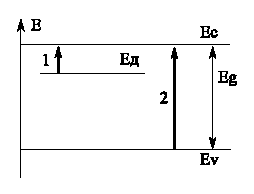
\includegraphics[height=4cm]{pic2_zone.eps}
\caption{Зонная диаграмма с одним типом донорной примеси}
\label{pic2_zone}
\end{figure}

\begin{figure}[h!]\centering
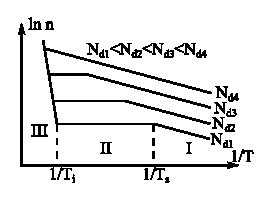
\includegraphics[height=4cm]{pic2_n_T.eps}
\caption{Общий вид температурной зависимости концентрации для невырожденного полупроводника с одним типом примеси}
\label{pic2_n_T}
\end{figure}

Из зависимости $\ln n = f(\frac{1}{T})$ можно выделить три характерных температурных интервала.

\paragraph{I. Область примесной ионизации.}
При абсолютном нуле валентная зона полупроводника целиком заполнена электронами. В зоне проводимости нет свободных носителей. При повышении температуры электроны переходят с уровней донорной примеси в зону проводимости, концентрация свободных электронов повышается. Это процесс называется ионизацией атомов примеси и продолжается вплоть до температуры истощения примеси $T = T_{s}$. В этой области
\begin{equation}
n = \sqrt{\frac{N_{c}N_{d}}{2}} \exp{\left( -\frac{E_{d}}{2 k T} \right)}
\label{eq2_n_T}
\end{equation}
где $N_{c} = 2 \left( \frac{2 \pi m_{dn}^{*} k T}{h^2} \right) ^ \frac{3}{2}$ - эффективная плотность состояний в зоне проводимости, $E_{d}$ - энергия ионизации донорной примеси, $N_{d}$ - концентрация примеси.

\paragraph{II. Область истощения примеси.}
В области температур $T_{s} < T < T_{i}$ донорная примесь полностью ионизована, но собственная ионизация ещё не началась. Поэтому концентрация свободных электронов постоянна и равна $N_{d}$.
Ширина области истощения зависит от концентрации ионизирующей примеси и её энергии ионизации. При увеличении этих величин температурный интервал области истощения будет уменьшаться. При достаточно больших значениях $N_{d}$ он может исчезнуть полностью.

\paragraph{III. Область собственной ионизации.}
В области высоких температур $(T > T_{i})$, когда энергия теплового движения электронов становится сопоставимой с шириной запрещённой зоны $(k T \approx E_{g})$, электроны начинают переходить из валентной зоны в зону проводимости, из-за чего концентрация свободных носителей резко возрастает. Происходит ионизация атомов основного вещеста.

\begin{equation}
n_{i} = \sqrt{N_{c} N_{v}} \exp{\left( -\frac{E_{g}}{k T} \right)} \sim T^{\frac{3}{2}} \exp{\left( -\frac{E_{g}}{k T} \right)}
\label{eq2_ni_T}
\end{equation}

Ширина запрещённой зоны также зависит от температуры. Для большинства полупроводников величина $E_{g}$ сложным образом снижается с температурой, однако в широком диапазоне температур она может быть аппроксимирована прямой линией:
\begin{equation}
E_{g}(T) = E_{g}(0) + \alpha T
\label{eq2_E_T}
\end{equation}
где $E_{g}(0)$ - значение, которое можно получить экстраполяцией температурной зависимости ширины запрещённой зоны на значение 0\textdegree К, $\alpha$ - температурный коэффициент изменения ширины запрещённой зоны, обычно отрицателен и составляет десятые доли мэВ/К.

На рисунке \ref{pic2_E_T} показана температурная зависимость ширины запрещённой зоны в кремнии.

\begin{figure}[h!]\centering
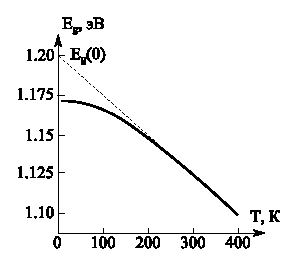
\includegraphics[height=4cm]{pic2_E_T.eps}
\caption{Температурная зависимость ширины запрещённой зоны для кремния}
\label{pic2_E_T}
\end{figure}

Подставляя (\ref{eq2_E_T}) в (\ref{eq2_ni_T}) получаем:
\begin{equation}
n_{i} = \sqrt{N_{c} N_{v}} \exp{\left( -\frac{E_{g}(0) + \alpha T}{k T} \right)} \sim T^{\frac{3}{2}} \exp{\left( -\frac{E_{g}(0)}{k T} \right)} \exp{\left( -\frac{\alpha}{k} \right)}
\label{eq2_ni_T}
\end{equation}

\subsection{Температурная зависимость подвижности СНЗ}
Подвижность также зависит от температуры. Характер зависимости определяется доминирующим механизмом рассеяния в полупроводнике при данной температуре. Для большинства механизсов зависимость $\mu(T)$ имеет ярко выраженную степенную зависимость:
\begin{equation}
\mu(T) = \mu_{i} \left( \frac{T}{T_{i}} \right)^{m}
\end{equation}
где $\mu_{i}$ - подвижность при температуре $T = T_{i}$.

Если основным механизмом является рассеяние на ионах примеси, показатель $m = \frac{3}{2}$. Для рассеяния на нейтральных примесях $m = 0$, а для рассеяния на акустических фононах $m = -\frac{3}{2}$. В реальных полупроводниках одновременно действует несколько механизмов рассеяния, поэтому определённое значение покащателя $m$ можно указывать только для ограниченного интервала температур. Для двух важнейших механизмов рассеяния - на акустических фононах и ионах примеси - температурная звисимость подвижности принимает вид, показанный на рисунке \ref{pic2_mu_T}

\begin{figure}[h!]\centering
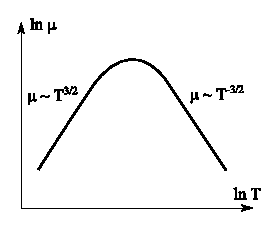
\includegraphics[height=4cm]{pic2_mu_T.eps}
\caption{Температурная зависимость подвижности свободных носителей заряда в невырожденном полупроводнике}
\label{pic2_mu_T}
\end{figure}

В области низких температур доминирующим механизмом рассеяния является рассеяние на ионах примеси. С ростом температуры подвижность увеличивается, так как увеличивается тепловая скорость носителей, и при взаимодействии с рассеивающими центрами (примеснми ионами) носители отклоняются на меньшие углы. С дальнейшим ростом температуры заметно возрастает амплитуда тепловых колебаний атомной решётки, и подвижность ограничивается рассеянием на акустических фононах, которое. При этом часто в реальных полупроводниках показатель подвижности для такого случая может отличаться от расчётного значения $m = -\frac{3}{2}$ в полтора раза в ту или другую сторону.

С учётом формул (\ref{eq2_n_T}) и (\ref{eq2_ni_T}) можно построить зависимость электропроводности от температуры. Примерный вид такой зависимости показан на рисунке \ref{pic2_sigma_T}.

\begin{figure}[h!]\centering
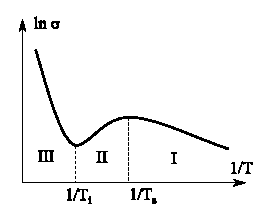
\includegraphics[height=4cm]{pic2_sigma_T.eps}
\caption{Температурная зависимость электропроводности в невырожденном полупроводнике}
\label{pic2_sigma_T}
\end{figure}

На приведённом графике можно выделить три области.

I. Область примесной проводимости
\begin{equation}
\sigma = e n(T) \mu(T) \sim T^{\frac{3}{4} + m} \exp{\left( -\frac{E_{d}}{2 k T} \right)}
\end{equation}

II. Область истощения примеси
\begin{equation}
\sigma = e N_{d} \mu(T) \sim N^{m}
\end{equation}

III. Область собственной проводимости
\begin{equation}
\sigma_{i} = e n_{i}(T) \left[ \mu_{n}(T) + \mu_{p}(T) \right] \sim T^{\frac{3}{2} + m} \exp{\left( -\frac{\alpha}{2 k} \right)} \exp{\left( -\frac{E_{g}(0)}{2 k T} \right)}
\end{equation}

У приведённой зависимости есть несколько характерных особенностей. В области истощения примеси температурная зависимость электропроводность определяется температурной зависимостью подвижности. В областях примесной и собственной ионизации большее влияние оказывает температурная зависимость концентрации носителей.

Если пренебречь слабой степенной зависимотью ширины запрещённой зоны от температуры, то области (I) и (III) имеют вид прямых с тангенсом угла наклона $-\frac{E_{d}}{2 k T}$ и $-\frac{E_{g}(0)}{2 k T}$ соответственно. Таким образом, экспериментальная зависимость логарифма проводимости от обратной температуры позволяет определить энергию ионизации и ширину запрещённой зоны полупровроводника. При этом стоит помнить, что величина $E_{g}(0)$ не равна в точности ширине запрещённой зоны в полупроводнике при температуре 0\textdegree К, а является точкой, в которой линейная аппроксимация зависимости для больших температур пересекает ось ординат. Ошибка при определении $E_{g}$ по такой аппроксимации может достигать единиц процентов.

\section{Методика измерения и описание установки}

В данной работе используется схема, приведённая на рисунке \ref{pic2_scheme}. Образец $R_{\text{обр}}$ включается в цепь последовательно с эталоном - высоким сопротивлением заранее известной величины $R_{\text{изм}}$. В ходе измерения через цепь пропускается ток, при этом падение напряжения на $R_{\text{обр}}$ и $R_{\text{изм}}$ снимается при помощи измерительного модуля Fractal MCX 52.1. Величина тока через образец $I_{\text{обр}}$ равна току через известное сопротивление и может быть найдена как
\begin{equation}
I_{\text{обр}} = I_{\text{изм}} = \frac{U_{\text{изм}}}{R_{\text{изм}}}
\end{equation}

\begin{figure}[h!]\centering
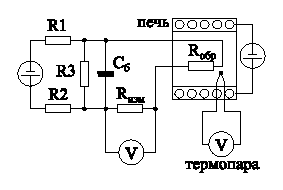
\includegraphics[height=4cm]{pic2_scheme.eps}
\caption{Принципиальная схема установки для измерения температурной зависимости электросопротивления}
\label{pic2_scheme}
\end{figure}

Так как наибольшей чувствительности сигма-дельта АЦП в составе модуля MCX достигает в диапазоне от $0.02$ до $2.56$ В, то в схеме используется делитель напряжения, построенный на резисторах $R1$, $R2$ и $R3$.

Чтобы исключить влияние термоЭДС, которая может возникнуть из-за градиента температуры вдоль образца, измерение производится короткими импульсами в двух направлениях. Конденсатор $C_{\text{б}}$ сглаживает возникающие пульсации, уменьшая уровень шума.

Образец в специальном держателе помещается в кварцевую трубку нагревателя, питание которого осуществляется от источника Э378. Температура образца измеряется термопарой, сигнал с которой автоматически пересчитывается измерительным модулем MCX 52. Результаты измерений падения напряжения на образце, эталонном сопротивлении и сигнал с термопары пересчитываются встроенным АЦП и передаются на компьютер, где по записанным в память уравнениям и калибровочным кривым пересчитываются в сопротивление измеряемого образца и температуру.

\section{Порядок проведения работы и указания по технике безопасности}

\begin{enumerate}
\item Запустить программу для измерения температурной зависимости электросопротивления.
\item Установить режим <<измерение>> и выбрать используемый в данной работе COM-port.
\item Запустить измерения и включить нагрев, подав 50В на нагреватель.
\item Нагреть образец до 120\textdegree C.
\item Выключить нагрев, охладить образец до 40\textdegree C.
\item Сохранить результаты измерения.
\end{enumerate}

Перед началом измерения необходимо убедиться в том, что защитный кожух и источник нпряжения заземлены. При работе с печью запрещается поднимать температуру выше 200\textdegree C.

\section{Обработка результатов эксперимента}

\begin{enumerate}
\item Результаты измерения занести в таблицу, отметив области нагрева и охлаждения.
\item Полученные значения построить в координатах $\ln \sigma = f \left( \frac{1}{T} \right)$.
\item На полученном графике (примерный вид приведён на рисунке \ref{pic2_experiment}) выделить два линейных участка, левый характеризует собственную проводимость, правая - примесную.
\item Наклон прямой определяется величиной энергии активации. В области собственной проводимости $\tg (\phi_{2}) = -\frac{E_{g}(0)}{2 k}$, откуда $E_{g}(0) = -2 k \tg(\phi_{2})$.
\item Аналогично определить энергию ионизацию примеси $E_{d} = -2 k \tg(\phi_{1})$.\
\item Определить ошибку измерения, определив энергию ионизации на различных участках кривой.
\end{enumerate}

\begin{table}[h!]
\caption{Измерение удельного электросопротивления при освещении (без освещения)}
\begin{center}
\begin{tabular}{c|c|c|c|c|c|c|c}
№ & $U$ & $t$ & $T$ & $R$ & $\sigma$ & $\ln(\sigma)$ & $\frac{1}{T}$ \\
\hline
& мВ & \textdegree C & К & Ом & $\text{Ом}^{-1} \text{см}^{-1}$ &  & K \\
\hline
\end{tabular}
\end{center}
\end{table}

\begin{figure}[h!]\centering
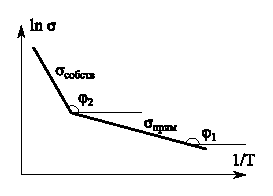
\includegraphics[height=4cm]{pic2_experiment.eps}
\caption{Типичный вид температурной зависимости электропроводности полупроводника}
\label{pic2_experiment}
\end{figure}

\section{Контрольные вопросы}

\begin{enumerate}
\item Понятие ширины запрещённой зоны и энергии ионизации примеси.
\item Температурная зависимость ширины запрещённой зоны в полупроводниках.
\item Температурная зависимость концентрации носителей для невырожденного полупроводника с явно выраженным типом проводимости.
\item Механизмы рассеяния носителей заряда в полупроводниках.
\item Температурная зависимость подвижности носителей заряд в полупроводниках.
\item Температурная зависимость электропроводности в полупроводниках.
\item Определение энергии активации примеси по температурной зависимости электросопротивления.
\item Основные факторы, ограничиваюие точность измерения.
\end{enumerate}

\section{Литература}

\begin{enumerate}
\item П.С. Киреев. Физик полупроводнико. М.: Высшая школа, 1975.
\item В.В. Горбачев, Л.Г. Спицина. Физика полупроводников и металлов. М.: Высшая школа, гл. 3, 1986 г.
\item Л.П. Павлов. Методы определения основных параметров полупроводниковых материалов. М.: Высшая школа, 1975 г.
\end{enumerate}